\chapter{Experimental field tests}
The autonomous landing system has successfully been tested in the field, where the result from two subsequent days is presented. The landing plan that was test was only with a virtual net that was placed $26$ meters above the ground, using guidance and high level control systems in DUNE. The navigation system used \gls{rtk-gps} with the compensator system enabled, which ensures that the positioning of the \gls{uav} can be assumed highly accurate. The result of the navigation system is presented in section \ref{ss:EXNavigation}.
\section{Landing system}
The wind condition the first day had an windspeed at $8-9 m/s$ from west, and the second day was calm wind conditions at $1 m/s$ from west. Hence the performance of system was tested with two different wind condition, where one strained the performance of the system while the other could be considered as ideal conditions. The virtual net was placed above a runway at Agdenes, such that the landing path is similar to a landing path where a physical net is used. All landing plan was generated when the \gls{uav} was in a loiter manoeuvre, such that the plan could be reviewed and the correct controllers assigned to the plan.
\subsection{Day 1}
The first plan created had the approach path cross the landing path, which lead the \gls{uav} into the crosswind on the straight line between the circles. This strained the lateral controller introduces oscillatory motion in the \gls{uav}. Figure \ref{Fig:NorthEast31mai103029} shows the lateral landing plan, including the flight path of the \gls{uav} and the position of the virtual net. Figure \ref{Fig:Height31mai103029} shows the desired height and the \gls{uav} height during the landing plan.

The behaviour of the lateral path shown in figure \ref{Fig:NorthEast31mai103029} indicates that the lateral guidance system is struggling to stay on the straight lines in the plan when flying in the crosswind. The oscillatory behaviour affect the path of the \gls{uav} when entering the final turning circle, where it overshoot the path. The overshot may cause the \gls{uav} to leave the line of sight of the pilot, which is a critical failure in a LOS flight operation. When entering the landing path the \gls{uav} continues to oscillate along the final straight line path, all though the \gls{uav} was able to have a cross track error at the time of passing the virtual net lower then the cross track error acceptance. The behaviour of the lateral behaviour can be increased by changing the rotation direction of the first turning circle, such that the straight line path between the circle do not cross the landing path. This will also allow the \gls{uav} to enter the final  turning circle at a better angle. The lookahead distance of the lateral controller can be reduced such that it will react more aggressive when flying in the head wind.

The longitudinal guidance system is able to follow it's reference, all though it is also struggling when attempting a glide slope decent in the head wind. However it  should be noted that the path shown in figure \ref{Fig:Height31mai103029} was constructed with a net impact angle of $\gamma_n = 3 \deg$, which resulted in the desired height failure to converge to the path due the smoothing filter introducing a constant bias from the desired path. In order for the desired height from the longitudinal guidance system to converge to the desired path the net impact angle $\gamma_n$ was set to zero. However this affect the total altitude descent along the landing path since now only the glide slope is used to reduce the altitude of the \gls{uav}. 
\newpage
\begin{figure}[H]
	\centering
		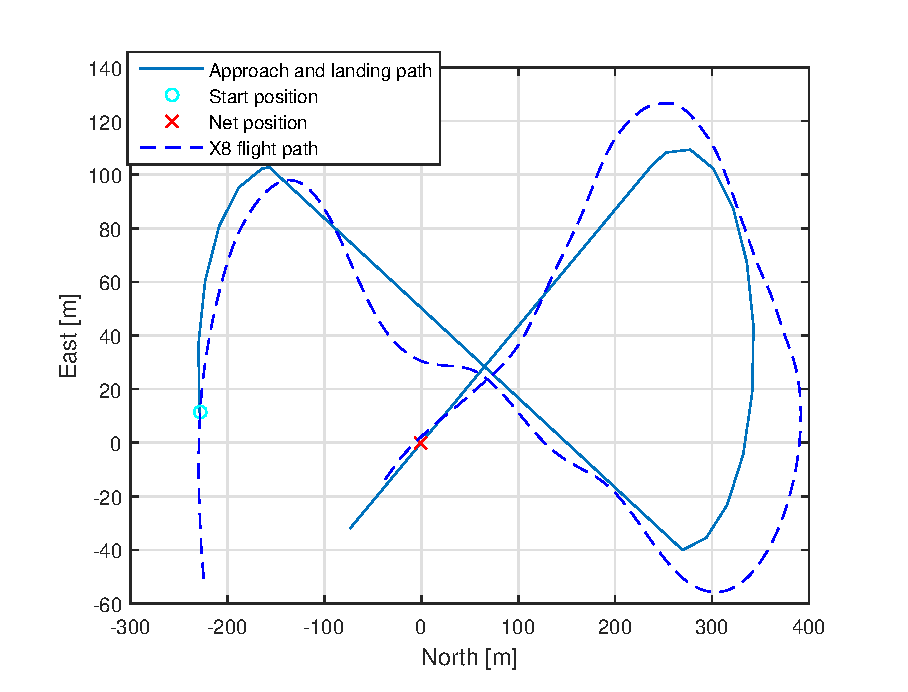
\includegraphics[scale=0.7]{figs/Experiment/NorthEast31mai103029.eps}
		\caption{North-East plot of a landing plan}
		\label{Fig:NorthEast31mai103029}
\end{figure}
\begin{figure}[H]
\centering
		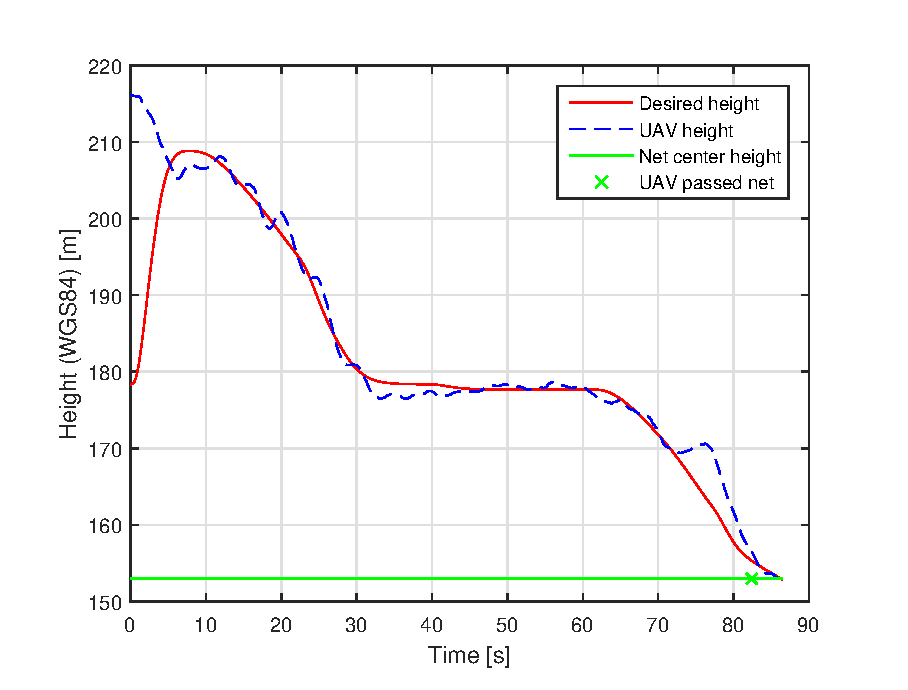
\includegraphics[scale=0.7]{figs/Experiment/Height31mai103029.eps}
		\caption{Height profile of landing plan with $3 \deg$ net impact angle}
		\label{Fig:Height31mai103029}
\end{figure}
A new landing plan, where the desired height and \gls{uav} during the landing plan is shown in figure \ref{Fig:Height31mai31mai105034}, was generated with the net impact angle $\gamma_n = 0$. The effect of setting the net impact angle to zero gave a better performance from the height guidance system. At the time the \gls{uav} passed the virtual net the hight error with respect the height of the net center was within the height error acceptance.

The minimum altitude that was used at the start of the landing path was set to $56 m$ above the runway. This is due to the length restriction of both the airfield and the operational area where the \gls{uav} is visible for the pilot. With the current landing plan and a landing direction from east the minimum height at which the \gls{uav} can starts its landing path is set to $56 m$ above ground. The effect of this requirement is discussed further in section \ref{sss:summaryDay1}.

During the new path the \gls{uav} was able to stay on the straight line towards the net. However the \gls{uav} still have oscillatory behaviour along the straight line connecting the two circles, with a large overshoot in the final turn. A better path would be to avoid flying in the cross wind as much as possible, which would result in a smoother path between the circles. However this will not remove the overshot in the final turn, all thought it will be reduced since the \gls{uav} is not in a oscillatory motion when entering the final circle.
\begin{figure}[H]
\centering
		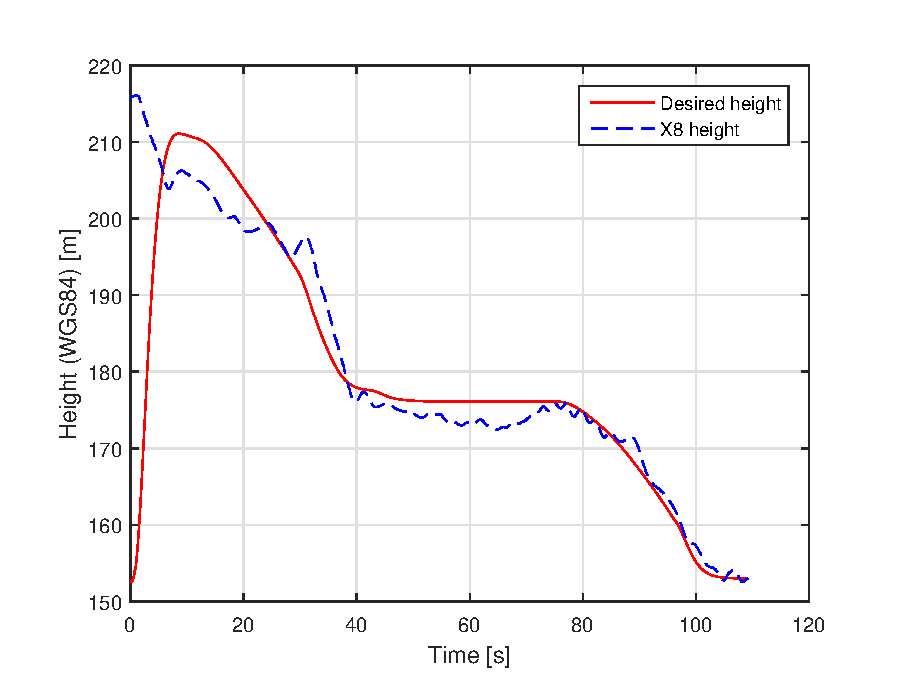
\includegraphics[scale=0.7]{figs/Experiment/Height31mai105034.eps}
		\caption{Height profile of landing plan with $0 \deg$ net impact angle}
		\label{Fig:Height31mai31mai105034}
\end{figure}
In order to reduce the oscillatory motion of the \gls{uav} a new path was constructed where the rotation direction of the first circle was changed to counter clockwise, as shown in figure \ref{Fig:NorthEast31mai125420}. The new path had its straight line path between the circles parallel to the wind direction, which resulted in less oscillatory motion and a smaller entry tangential angle into the final turning circle. However the overshoot in the final circle is still present, and is a result of the \gls{uav} attempting to turn up against the wind. The oscillatory motion was reduced by changing the rotation direction of the first turning circle, however the \gls{uav} is still not able to stay on the straight line paths in the landing plan. 
\begin{figure}[H]
	\centering
	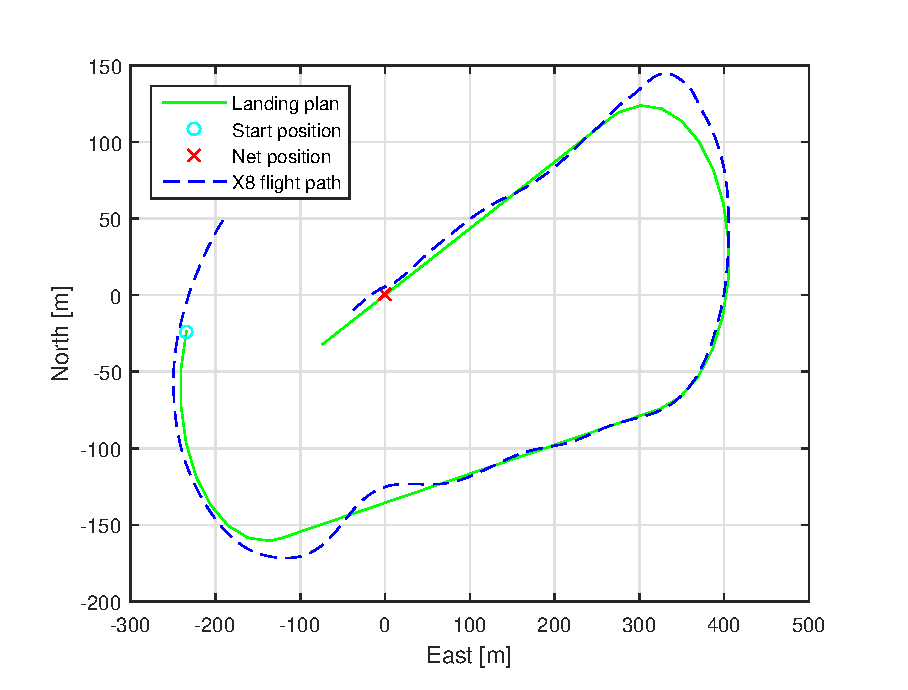
\includegraphics[scale=0.7]{figs/Experiment/NorthEast31mai125420.eps}
	\caption{North-East plot where the straight line segment between the two circles give a path parallel to the wind}
	\label{Fig:NorthEast31mai125420}
\end{figure}
In order to further reduce the oscillatory motion of the lateral controller the lookahead distance was reduced to make the controller more aggressive towards the wind. The effect of this change is shown in figure \ref{Fig:NorthEast31mai131844}, where the oscillatory motion is almost completely removed. However the overshot at end of the final circle indicates that the lateral controller is struggling to handle a turning circle. 
\begin{figure}[H]
\centering
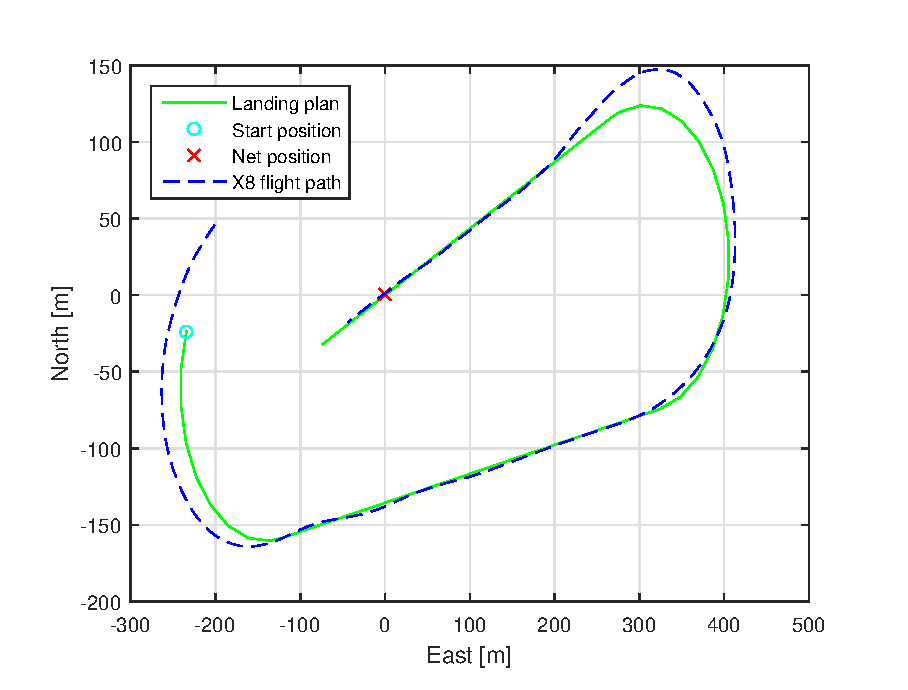
\includegraphics[scale=0.7]{figs/Experiment/NorthEast31mai131844.eps}
\caption{North-East plot where the lookahead distance of the lateral controller was reduced to increase performance when flying against the wind}
\label{Fig:NorthEast31mai131844}
\end{figure}
Looking at the desired roll ($\phi_d$ ) and the actual roll ($\phi$) of the \gls{uav} at the time of the final turn, shown in figure \ref{Fig:DesiredRoll131844}, it's observed that the controller does not try to keep a constant bank through the turn. Instead it lowering the roll angle, which in turn affect the performance of the \gls{uav} at the end of the turn. The performance might be reduced by reducing the distance between each arc segments in the turning circle, and experimenting with the radius of the turning circle. However this was not attempt during the first day, all thought attempts to reduce overshot by lowering the distance between each arc segments was performed the following day.
\begin{figure}[H]
\centering
\includegraphics[scale=0.7]{figs/Experiment/rollDesired131844.eps}
\caption{The desired roll and actual roll of the \gls{uav}}
\label{Fig:DesiredRoll131844}
\end{figure}
\subsubsection{Summary of day 1}\label{sss:summaryDay1}
The result from the first day was affected with strong wind condition, in which the \gls{uav} struggled to stay on the path. The mean height and cross track error is listed in table \ref{tb:Day1HeightCrossTrack}, where the first column indicate the number of the landing attempt. As seen in table \ref{tb:Day1HeightCrossTrack} the average cross track error equals to $5.4 m$
\begin{table}[H]
\centering
\begin{tabular}{| l | l | l |}
\hline
\textbf{Nr.} 	& \textbf{Average height error [m]} 	& \textbf{Average cross track error [m]}  \\ \hline
$1$				& $1.5$							& $6.1$								\\ \hline
$2$				& $2.6$							& $6.7$								\\ \hline
$3$				& $0.9$							& $5.5$								\\ \hline
$4$				& $0.1$							& $2.8$								\\ \hline
$5$				& $1.7$							& $2.0$								\\ \hline
$6$				& $1.3$							& $6.8$								\\ \hline
$7$				& $1,8$							& $9.1$								\\ \hline
$8$				& $1.2$							& $8.2$								\\ \hline
$9$				& $1.9$							& $5.9$								\\ \hline
$10$			& $1.5$							& $4.4$								\\ \hline
$11$			& $1.5$							& $1.4$								\\ \hline
Average				& $1.5$							& $5.4$								\\ \hline
\end{tabular}
\caption{Mean height and cross track error from day 1}
\label{tb:Day1HeightCrossTrack}
\end{table}
The longitudinal guidance system was able to keep a stable average height error during the landing plans. However the longitudinal control system must be further fine tuned in order to achieve the precision needed to perform a autonomous landing during windy conditions. A table containing if a landing plan would result in a net landing is presented in table \ref{tb:Day1LandingAttempt}. The success rate of the first day gives a $36.3  \% $ probability of successfully landing in the net, which indicate that alteration to the current landing system is needed in order to achieve better performance in strong wind conditions.
\begin{table}[H]
\centering
\begin{tabular}{| p{0.5cm} | p{1cm} | p{1cm} | p{3.5cm} | p{3cm} | p{1cm} |}
\hline
\textbf{Nr.}	& \textbf{Height error [m]}	& \textbf{Cross track error [m]}& \textbf{Height acceptance}& \textbf{Cross track error acceptance}	& \textbf{Net hit}\\ \hline
$1$				& $2.8$		& $2.1$		& X								& OK									& X					\\ \hline
$2$				& $2.7$		& $-4.5$	& X								& X										& X					\\ \hline
$3$				& $0.9$		& $-1.6$	& OK							& OK									& OK				\\ \hline
$4$				& $0.0$		& $5.4$		& OK							& X										& X					\\ \hline
$5$				& $0.8$		& $5.3$		& OK							& X										& X					\\ \hline
$6$				& $2.1$		& $-1.6$	& X								& OK									& X					\\ \hline
$7$				& $0.7$		& $2.3$		& OK							& OK									& OK				\\ \hline
$8$				& $-1.5$	& $-5.4$	& X								& X										& X					\\ \hline
$9$				& $1.9$		& $0.8$		& X								& OK									& X					\\ \hline
$10$			& $0.3$	& $1.1$		& OK							& OK									& OK				\\ \hline
$11$			& $-1.3$	& $0.2$		& OK							& OK									& OK				\\ \hline
\end{tabular}
\caption{Table containing the result of each landing attempt}
\label{tb:Day1LandingAttempt}
\end{table}
The content of table \ref{tb:Day1LandingAttempt} is shown in figure \ref{Fig:Day1NetPass}, where the net is marked as a whole line and all landing attempts are marked as crosses. The osilatory motion in the lateral plane by the \gls{uav} is reflected in the placement of the crosses. However the placement of the cross is evenly divided along the cross track error axis, which is not reflected in the placement along the height error axis. The placement along the height error axis indicates that the \gls{uav} 
\begin{figure}[H]
\centering
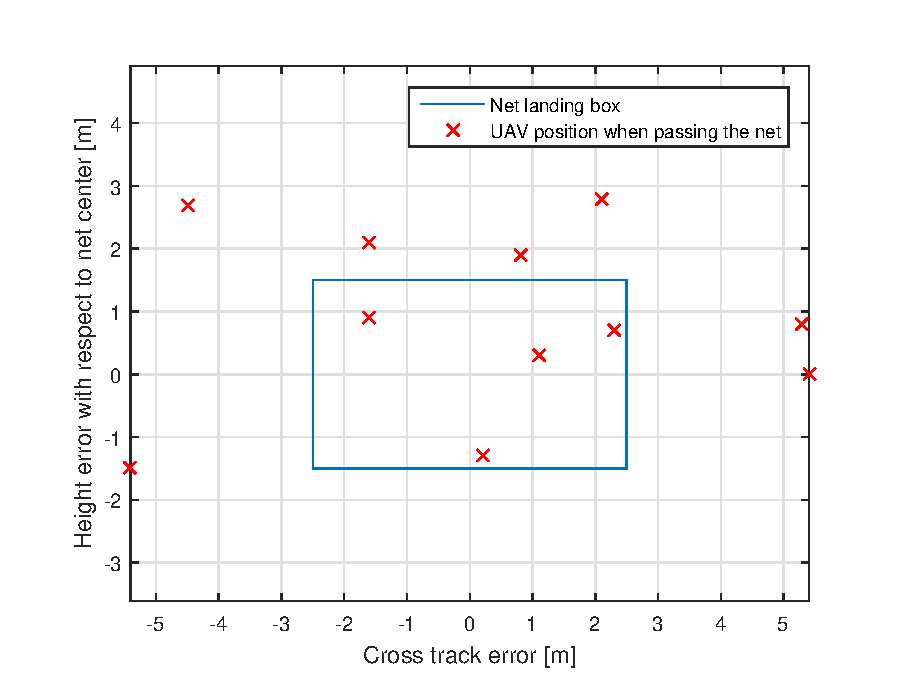
\includegraphics[scale=0.7]{figs/Experiment/day1NetHit.eps}
\caption{Position of UAV relative to the net center at the time of net passing}
\label{Fig:Day1NetPass}
\end{figure}
The maximum length of the landing path with the radius of the final turning circle must be within the flight operation area. On Agdenes when attempting to land from the East the restriction is estimated to be $700 m$, with minimum altitude of $56 m$. 
\begin{table}
\centering
\begin{tabular}{| p{2cm} | p{4cm} | p{2cm} | p{2cm} |}
\hline
\textbf{Net offset [m]}	& \textbf{Needed decent height [m]}& \textbf{Glide slope length [m]}& \textbf{Glide slope angle [$\deg$]}	\\ \hline
$0$						& $56$													&$700$							& $4.6$			\\ \hline
$3$						& $53$													&$700$							& $4.3$			\\ \hline
$3$						& $53$													&$300$							& $9.5$			\\ \hline
\end{tabular}
\caption{Different decent heights and length of glide slope with responding glide slope angle}
\label{Tb:GlideSlopeAngles}
\end{table}
The minimum altitude will vary if the \gls{uav} can start its landing path from the west, however this will only be the case during calm wind condition or a wind direction from the east. In addition increased glide slope angle will result in the \gls{uav} to build up speed, however decreasing the throttle in order to reduce lift might be a method used to quickly lose hight during the landing path.
\subsection{Day 2}
The second day had calm wind condition, which is considered as ideal field test conditions for the autonomous landing system. For the new landing plan the virtual net was moved in order for the landing path to use more of the runway. In addition the heading of the net was changed such the landing path became parallel to the runway. The main goal with the flight today was to reduce to overshot in the final turn, and to investigate how to increase the performance of the height guidance system. To increase the height difference between the net center and the start of the landing path both the length of the glide slope and glide slope angle was increased.

The path generated with the new parameters is shown in figure \ref{Fig:NorthEast1juni081328}. The lateral path overshoots in both the start and final turning circles. As seen in figure \ref{Fig:Roll1juni081328} the roll motion of the \gls{uav} does not follow the desired roll, which is due to the low level roll controller is tuned for manual flight where rapid changes in the actuators is undesired. In addition the control surface used to control the roll of the \gls{uav} is also used to control the pitch, which results in having to weight the performance in heading against the ability to follow a height reference.
\begin{figure}[H]
\centering
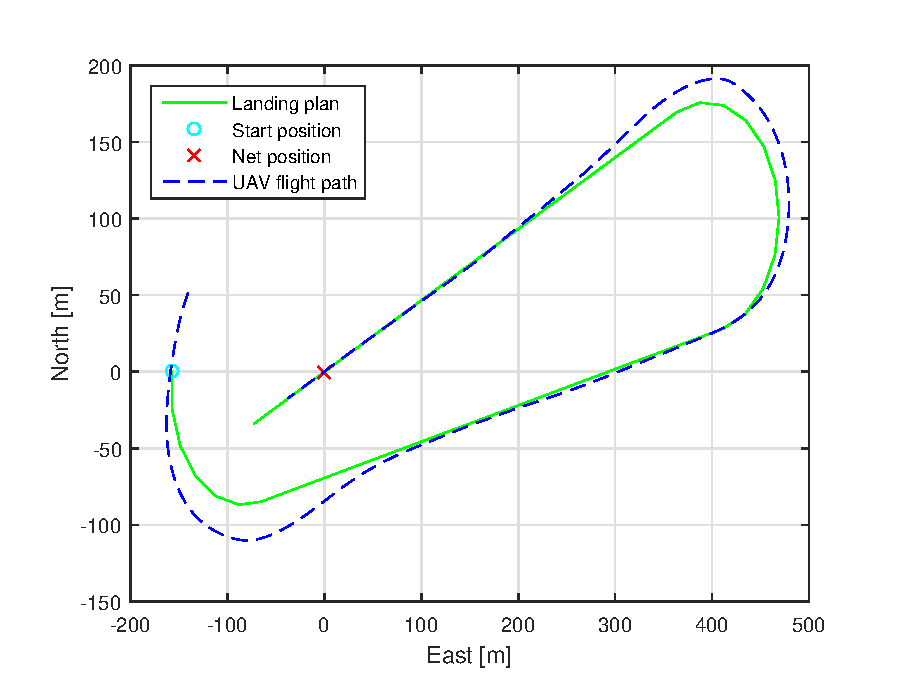
\includegraphics[scale=0.7]{figs/Experiment/NorthEast1juni081328.eps}
\caption{North-East plot}
\label{Fig:NorthEast1juni081328}
\end{figure}
\begin{figure}[H]
\centering
\includegraphics[scale=0.7]{figs/Experiment/Roll1juni081328.eps}
\caption{Roll}
\label{Fig:Roll1juni081328}
\end{figure}
The resulting desired height and \gls{uav} height from the new path, shown in figure \ref{Fig:Height1juni081328}, shows that the \gls{uav} was unable to follow a glide slope with glide slope angle $\gamma_l = 8 \deg$. A major reason for this behaviour is due to the failure of the \gls{uav} pitch to follow the desired pitch, as shown in figure \ref{Fig:Pitch1juni081328}. The pitch appear to to saturated in the low level controller since it does not reach the desired pitch. Better tuning of the low level control system might reduce the bias and lag between actual and desired pitch value, however the reason for the saturation must be further investigated. A restriction in the desired pitch available for the control system, indicate that a new strategy is need in a autonomous landing system where speed assignment during the landing path must be investigated.
\begin{figure}[H]
\centering
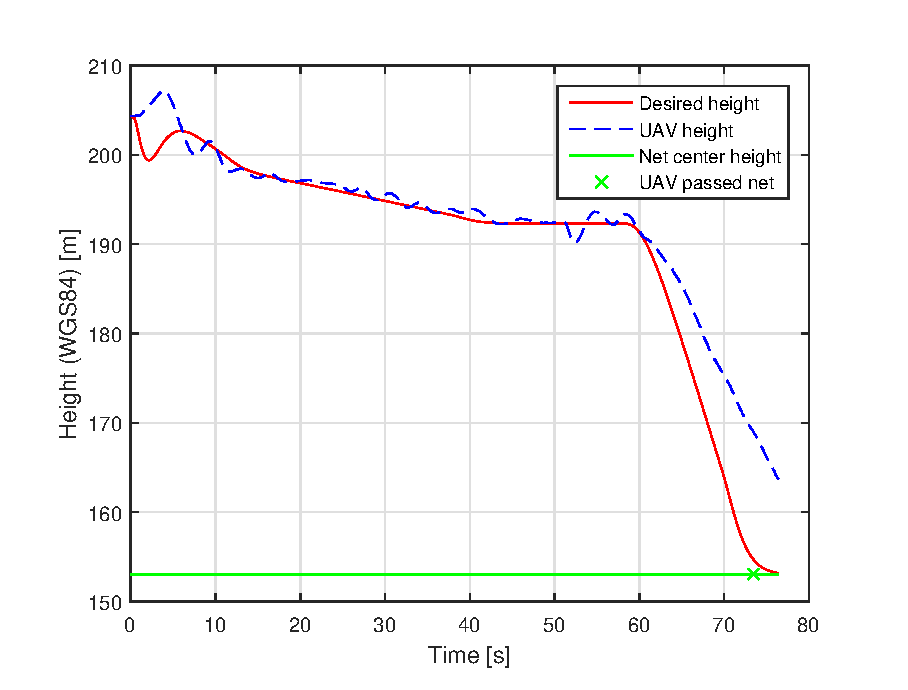
\includegraphics[scale=0.7]{figs/Experiment/Height1juni081328.eps}
\caption{Height}
\label{Fig:Height1juni081328}
\end{figure}
\begin{figure}[H]
\centering
\includegraphics[scale=0.7]{figs/Experiment/Pitch1juni081328.eps}
\caption{Pitch}
\label{Fig:Pitch1juni081328}
\end{figure}
In order to reduce the overshot in the final turning circle the distance between each arc segments each turning circle was reduced. The goal for with this alteration was to get the lateral controller to keep the roll angle in order to increase the turning performance. Figure \ref{Fig:NorthEast1juni083423} shows the the resulting path when the arc segment distance is reduced. The overshot in the final turning circle is reduced, and the cross track error in the final turning circle is shown in figure \ref{Fig:CrossTrackError1juni083423} indicates that the performance of the \gls{uav} increase with short distance between arc segments. A long term solution for reducing overshot in a turning circle would be a dedicated controller for turning manoeuvre. If combined with the current lateral controller which is designed to stay on a straight line between way-point the result will be a controller that is well suited for performing a autonomous landing.
\begin{figure}[H]
\centering
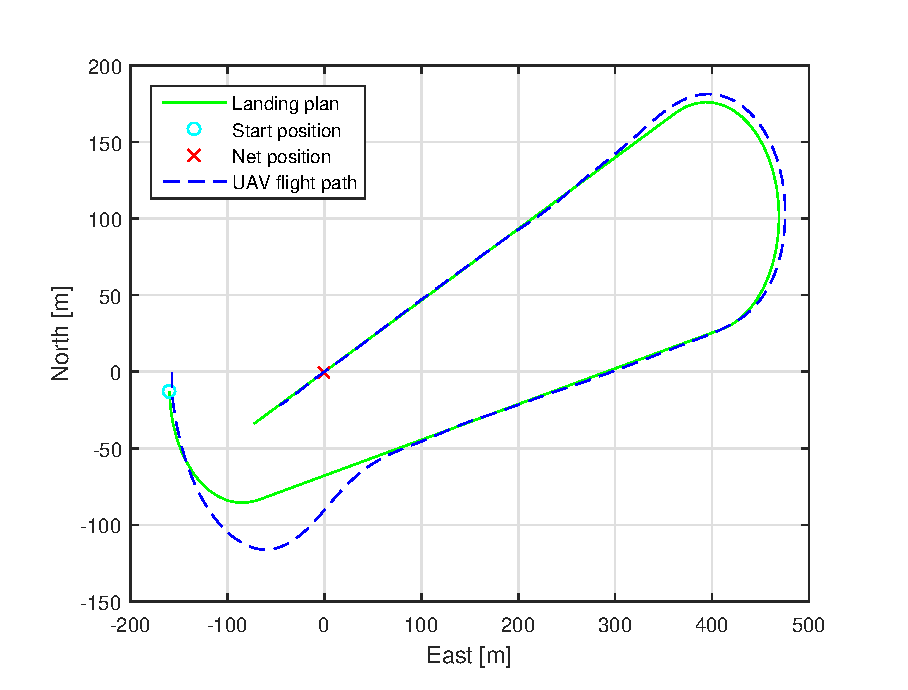
\includegraphics[scale=0.7]{figs/Experiment/NorthEast1juni083423.eps}
\caption{North-East plot where the distance between each arc segments has been reduced from $25 m$ to $10 m$}
\label{Fig:NorthEast1juni083423}
\end{figure}
\begin{figure}[H]
\centering
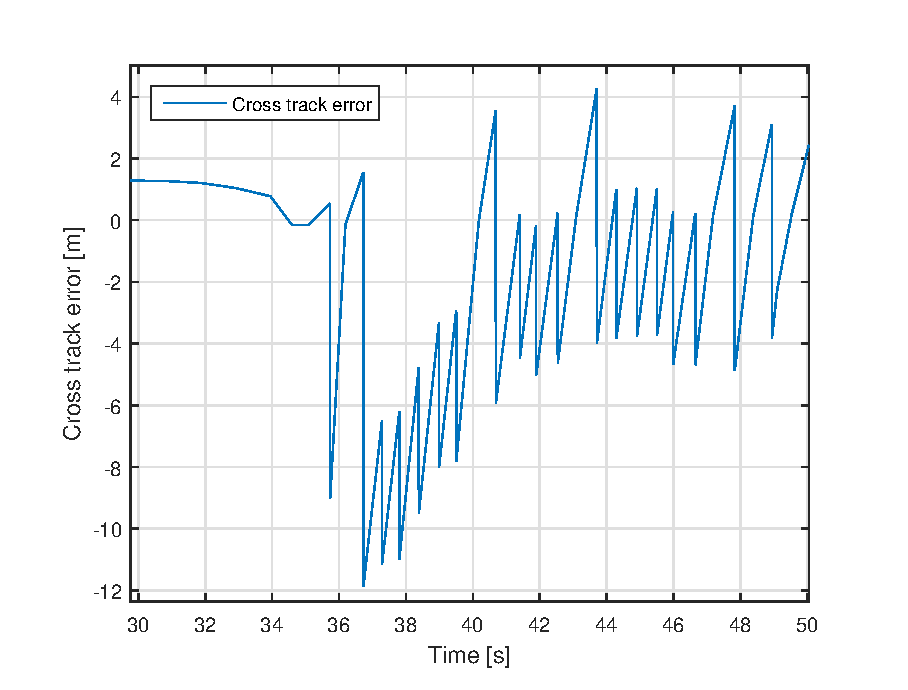
\includegraphics[scale=0.7]{figs/Experiment/CrossTrackError1juni083423.eps}
\caption{Cross track error in the final turning circle}
\label{Fig:CrossTrackError1juni083423}
\end{figure}
\subsubsection{Summary day 2}
The second day had more experimental testing then the first day, where the limits of the height profile and reducing the overshoot in the final turning circle was the main focus. The testing of limits for glide slope angle is reflected in table \ref{Tb:AverageCrossHeightDay2} where the net misses is due to height error. With the current system the limit was found to be $\gamma_l=6\deg$, however better tuning of low level pitch controller and reducing landing speed could increase the limitation on the glide slope angle. The short final approach length resulted in the \gls{uav} to have a short distance of which the net center height could be reached. A longer final approach would result in a higher success rate, however this would require either a longer landing path or shorter glide slope. The final approach could be increased to $120 m$ by moving the net further west over. The risk with a large final approach during a autonomous landing in a real net would be the prolonged time the \gls{uav} flies $3-4 m$ above ground. A loss of high accurate positioning system could then result in a crash.
\begin{table}[H]
\centering
\begin{tabular}{| p{0.5cm} | p{1cm} | p{1cm} | p{3.5cm} | p{3cm} | p{1cm} |}
\hline
\textbf{Nr.}	& \textbf{Height error [m]}	& \textbf{Cross track error [m]}& \textbf{Height acceptance}& \textbf{Cross track error acceptance}	& \textbf{Net hit}\\ \hline
$1$				& $14.4$		& $0.1$		& X								& OK									& X					\\ \hline
$2$				& $1.3$		& $0.6$	& OK								& OK										& OK					\\ \hline
$3$				& $1.1$		& $-0.2$	& OK							& OK									& OK				\\ \hline
$4$				& $1.4$		& $0.1$		& OK							& OK										& OK					\\ \hline
$5$				& $1.1$		& $0.1$		& OK							& OK										& OK					\\ \hline
$6$				& $2.0$		& $-0.2$	& X								& OK									& X					\\ \hline
$7$				& $2.3$		& $0.2$		& X							& OK									& X				\\ \hline
$8$				& $7.0$	& $0.3$	& X								& OK										& X					\\ \hline
\end{tabular}
\caption{Table containing the result of each landing attempt}
\label{tb:Day2LandingAttempt}
\end{table}
\begin{figure}[H]
\centering
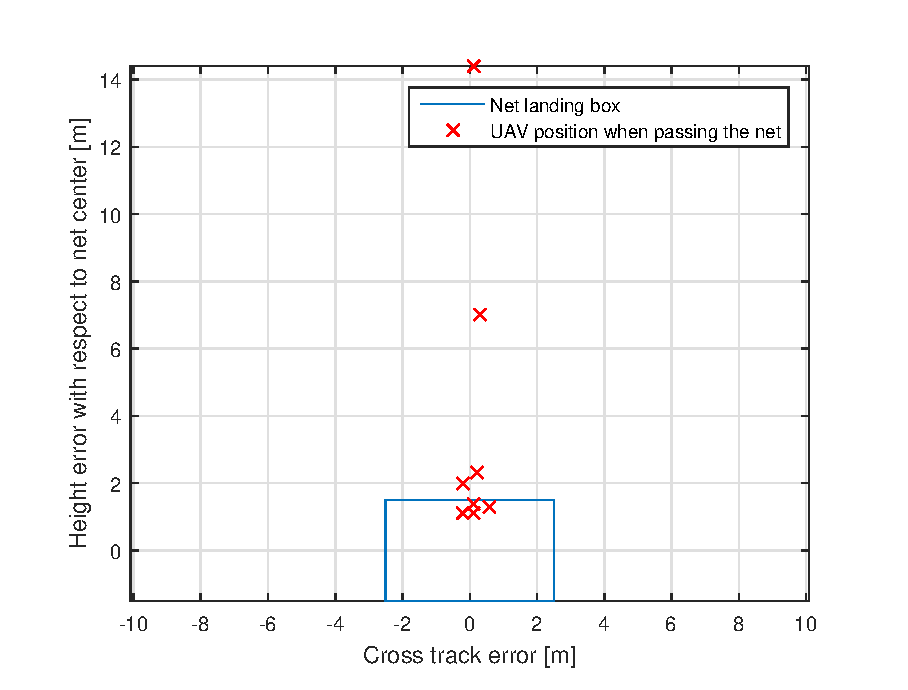
\includegraphics[scale=0.7]{figs/Experiment/day2NetHit.eps}
\caption{Position of the \gls{uav} relative to the net center at the time of net passing}
\label{Fig:Day2NetPass}
\end{figure}
The performance of the lateral controller increase during calm wind condition, however the performance of the longitudinal controller is the same as during windy conditions. Table \ref{Tb:AverageCrossHeightDay2} list up the average height error and cross track error relative to the desired height and path. 
\begin{table}[H]
\centering
\begin{tabular}{| l | l | l |}
\hline
\textbf{Nr.} 	& \textbf{Average height error [m]} 	& \textbf{Average cross track error [m]}  \\ \hline
$1$				& $2.2$							& $3.8$										\\ \hline
$2$				& $1.2$							& $3.4$										\\ \hline
$3$				& $0.9$							& $-1.8$									\\ \hline
$4$				& $2.5$							& $-0.2$									\\ \hline
$5$				& $3.0$							& $0.3$										\\ \hline
$6$				& $1.6$							& $0.2$										\\ \hline
$7$				& $1,9$							& $-2.3$									\\ \hline
$8$				& $1.9$							& $-0.1$									\\ \hline
\end{tabular}
\caption{Average height and cross track error from day 2}
\label{Tb:AverageCrossHeightDay2}
\end{table}
\section{Navigation}\label{ss:EXNavigation}
The testing of the navigation system is restricted to the X8, however the same navigation system was used in a multicoper \gls{uav} both days.
\subsection{RTK-GNSS performance}
The performance of the \gls{rtk-gnss} system during the first day of executing landing plans is summaries in table \ref{TB:RTKFirstDayRTK}, which shows that \gls{rtk-gnss} kept a stable FIX during the landing plan experiment. The same result was achieved during the second day during the execution of the landing plans, however the \gls{rtk-gps} experienced problem later the second day, due to lost contact with the base station. The expected reason is that pore satellite geometry made effective use of \gls{rtk-gps} difficult.
\begin{table}[H]
\centering
\begin{tabular}{| l | l | l | l |}
\hline
\textbf{Nr.}	& \textbf{FIX \%}	& \textbf{FLOAT \%}	& \textbf{NONE \%}	\\ \hline
$1$				& $99.5 $	& $0.5$	& $0.0$									\\ \hline
$2$				& $99.5 $	& $0.5$	& $0.0$									\\ \hline
$3$				& $99.8 $	& $0.0$	& $0.0$									\\ \hline
$4$				& $100$		& $0.0$	& $0.0$									\\ \hline
$5$				& $100$		& $0.0$	& $0.0$									\\ \hline
$6$				& $100$		& $0.0$	& $0.0$									\\ \hline
$7$				& $99.9$	& $0.1$	& $0.0$									\\ \hline
$8$				& $99.7 $ 	& $0.3$	& $0.0$									\\ \hline
$9$				& $99.3$	& $0.7$	& $0.0$									\\ \hline
$10$			& $100$		& $0.0$	& $0.0$									\\ \hline
$11$			& $100$		& $0.0$	& $0.0$									\\ \hline
\end{tabular}
\caption{Performance of the RKT-GNSS system the first day during the executing of the landing plans}
\label{TB:RTKFirstDayRTK}
\end{table}
\subsection{Short loss compensator}
The short loss compensator was designed to prolong the availability of the \gls{rtk-gps}, such that a flight plan does not get interrupted due to a temporary problem with the \gls{rtk-gnss}. During a flight the second day the gls{rtk-gps} experienced a short drop out, as seen in figure \ref{Fig:NavSource}. Even though the \gls{rtk-gps} position solution is unavailable the navigation system is still able to supply high accurate position solution due to the short \gls{rtk-gnss} compensator as seen in figure \ref{Fig:ShortLoss}. The duration of the short \gls{rtk-gps} could be expanded, and currently the time limitation of the compensator where the position solution start to diverge is unknown.
\begin{figure}[H]
\centering
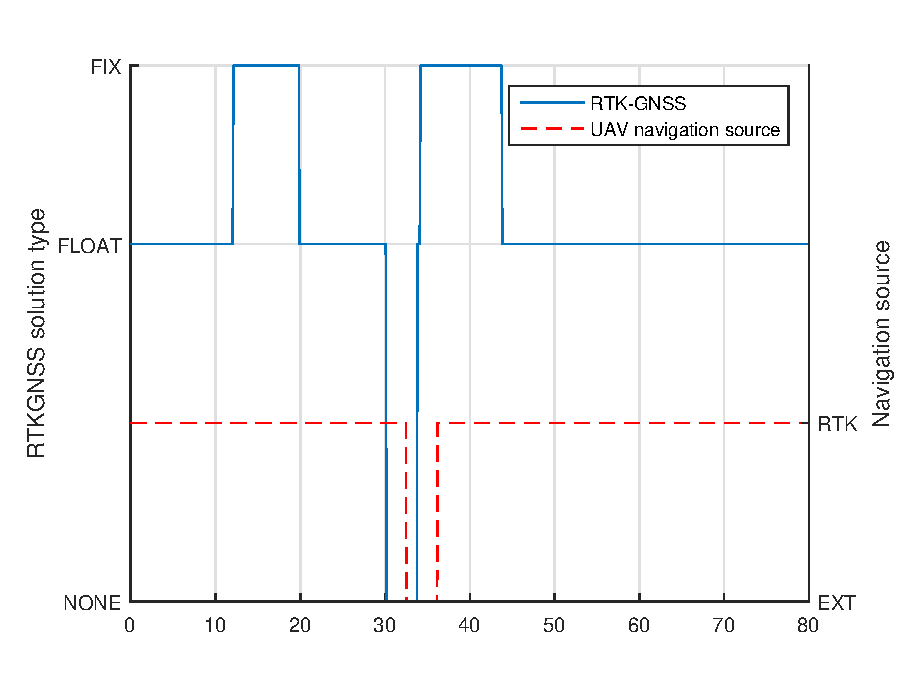
\includegraphics[scale=0.7]{figs/Experiment/navSource.eps}
\caption{State of RTK-GNSS system and \gls{uav} navigation source.}
\label{Fig:NavSource}
\end{figure}
\begin{figure}[H]
\centering
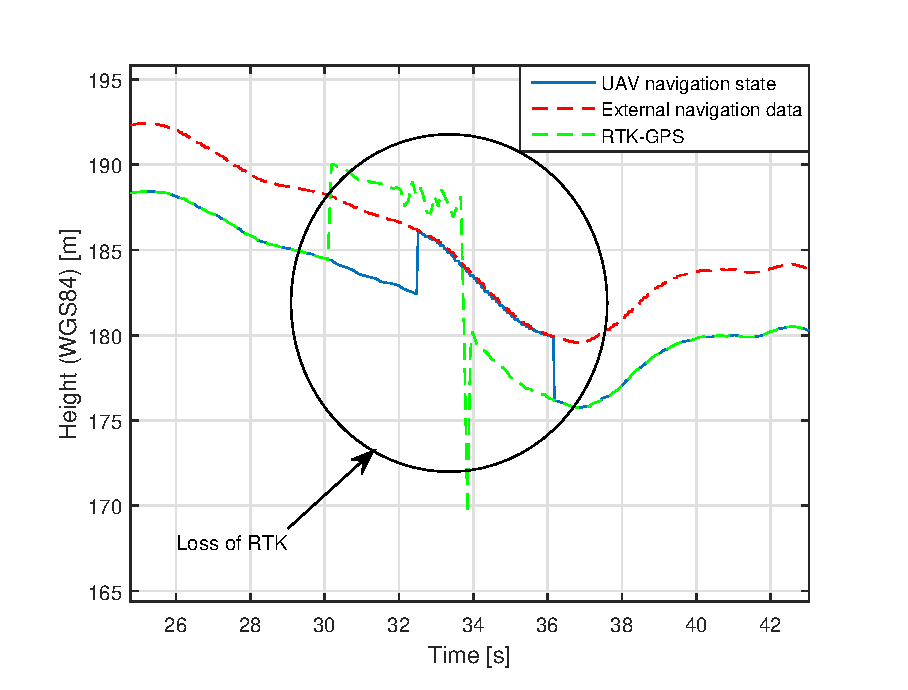
\includegraphics[scale=0.7]{figs/Experiment/shortrtkloss1juni114124.eps}
\caption{Loss of \gls{rtk-gps} triggers the short loss compensator such that the \gls{uav} keeps the \gls{rtk-gps} position solution longer}
\label{Fig:ShortLoss}
\end{figure}
\section{Summary}
This chapter showed the performance of a X8 fixed wing \gls{uav} performing a autonomous landing in a virtual net. The performance of the navigation system is acceptable for a autonomous system by supplying a stable highly accurate position solution, with redundancy for short \gls{rtk-gps} loss periods. The landing plan still require further testing to develop path parameters that  will result in a successful net landing. The path parameters are depending on the ability for the control system to follow the desired path, which might prove demanding in the longitudinal plane for large change in high over a short distance.